\chapter{Analysis and Design} \label{chap:analysis_and_design}

This chapter outlines overall design for the project as well as the analysis that form the basis of each decision. The design of the project is mostly guided by the requirements set out at the start of the chapter. The choice programming language and software/hardware tools, the processing of each dataset, and finally the structure of various novel classification pipelines are all set out before the implementation part of the report. As well as this a new frame-integration method is proposed, as well as state-of-the-art classification networks. The final part of this chapter also creates a framework for the comparison of each network, which can be found in \cref{chap:testing_and_results} and \cref{chap:evaluation}.

\section{Hardware and Software}

\subsection{Programming Languages}

When choosing a programming language for the project there were a few choices that are most often chosen by developers; Python\cite{Python}, R\cite{R}, and C++\cite{C++}. Python is the most popular choice due to the ease with which algorithms can be developed using it. Python features an extensive list of libraries and debugging functions that are invaluable when creating machine learning algorithms in particular, making the language of choice for this project. It is also important to note, however, the benefits of the other language options. C++ often results in programs with impressive performance due to the ability it grants to make low-level processes more efficient. Unfortunately this fine-level control also opens up programmers to more a demanding and time-intensive programming experience, with much more code writing and debugging to be done manually. R would also be a great choice for machine learning, and shares many similarities with Python, being open-source and having a huge community of developers constantly building libraries and tools. It has a different approach to machine learning, with a a more statistical analysis emphasis. Therefore Python remains the best choice for a more general approach for data processing.

\subsection{Machine Learning Frameworks and Software}

\subsubsection{PyTorch}

Pytorch\cite{Pytorch} is a relatively new framework for machine learning, and provides a developer friendly way to write machine learning code. It is a more `pythonic' approach to code abstraction that its competition in the space, and the \emph{torch.nn.module} gives access to clear, reusable module definitions in an Object-Oriented Programming manner. It also allows for simple data parallelism, so that batch processing can easily be split over different sets of hardware. It also has an intuitive debugging experience since itt can use standard debugging tools such as PyCharm and pdb.

\subsubsection{Tensorflow}

Tensorflow\cite{Tensorflow} is the older and more widely adopted machine learning library. It provides a more robust set of functionality with clear documentation. In terms of deployment it is the clear favourite as it allows models to be deployed on specialised servers and even on mobile. When visualising data software such as TensorBoard are ideal as it includes functionality to display model graphs, variables, histograms and much more. As well as this, Keras\cite{Keras} is a framework developed by Google, and uses a primarily Tensorflow based back-end. It provides an easy to use API for fast prototyping abd high levels of abstraction. It is used commercially by a plethora of companies and has a vast and highly developed research community. For these reasons Keras using a Tensorflow back-end were chosen for this project.

\subsection{Other Software}

\subsubsection{SpikingJelly}

SpikingJelly\cite{SpikingJelly} is an open-source deep learning framework for Spiking Neural Network (SNN) based on PyTorch. It allows for the processing of many often-used datasets in the neuromorphic community (Some of which are described in \cref{sec:existing_datasets}), as well as a simple set of classes for building SNNs or converting ANNs to SNNs. The library, which was mainly co-developed by Multimedia Learning Group, Institute of Digital Media (NELVT), Peking University and Peng Cheng Laboratory, can be installed directly via the \emph{pip} command. Using it, data can be loaded as event streams, as well as integrated frames (described in \cref{ssec:frame_integration}) of varying frame lengths or frame-rates. As well as this the package features clear documentation and tutorials to begin analysing neuromorphic data.

\subsubsection{NengoDL} \label{sssec:nengo}

NengoDL\cite{NengoDL} is a software framework designed to combine the strengths of neuromorphic modelling and deep learning. It is a useful tool for constructing biologically inspired spiking neuron models, and combining them to create fully spiking neural networks. As well as these these networks are intermixed with efficiently simulated deep learning concepts such as convolutional neural networks. This unified framework therefore allows us to train SNNs in the same way as we would for other ANN models with an easy to use interface. As well as this converters exist in order to convert ANNs to SNNs with relative ease.

\color{red} TODO: This could be moved if Nengo doesn't end up being used. \color{black}

\subsection{Cloud Environments}

Since Python is the language of choice for the project, Python Notebooks are a good choice for code segmentation and presentation. They allow for python code to be written in executable cells, so that their output as well as other text can be presented in a full document. This makes the code easy to understand for others, and good for development as well. Python notebooks can be run locally on a web server, as well as online on a cloud service. Many machine learning frameworks and algorithms make use of hardware acceleration using GPUs or TPUs. This means that code runs much faster on more powerful machines with this specialised hardware in them, which was not the case for hardware readily available during the course of the project. For this reason cloud services provided by the likes of Google and Amazon Web Services are a good alternative to physically owning hardware. They allow for the renting of GPUs etc. from their own servers, so that code can be run on them via their respective web services. 

The two main web services available at this time are Google Colaboratory\cite{GoogleColab} and AWS Sagemaker Studio Lab\cite{AwsSagemaker}. In terms of hardware, both services offer access to great GPUs, though sagemaker offers the more powerful T4 GPU at the free tier. This benefit, however, is not entirely relevant as a pro subscription would be necessary with either service to make use high-RAM runtimes. Due to Colaboratory's better share-ability and wider adoption, it was chosen as the service for this project.

\section{Datasets}

The datasets used for the evaluation of the networks in this project were NMNIST (\Cref{sssec:nmnist}), DVS128 Gesture (\Cref{sssec:dvs128_gesture}) and CIFAR10-DVS (\Cref{sssec:cifar10_dvs}), since these are the most suited for training on classification tasks. As well as this their recording conditions and topics are varied, meaning an evaluation of the system can be more robust and reliable. The event camera dataset for slam (\Cref{sssec:event_camera_dataset}) are also extensive and include side by side frames from a traditional camera, and so were ideal to use for testing the event reconstruction algorithms.

\subsection{Data Pre-processing} \label{ssec:data_preprocessing_design}

Before processing it, z-score standardisation needs to take place. \Cref{eq:z_score} shows the equation dictating the process. In practical terms the standard deviation of $ x $ can be substituted by the max value of $ x $. The reason this needs to occur is to `center' the data, meaning the inputs to the network can be guaranteed to be of a certain scale. In the training process the weights and biases (as described in \cref{eq:artificial_neuron_output}) are applied to the initial inputs, which are then back-propagated based on the loss gradient. The standardisation process ensures that these gradients don't spike out of proportion, meaning the same global learning rate can be used for the network. As well as this parameters are often shared across deep learning networks, and if inputs weren't of a similar scale for every part of an image, then this sharing of parameters wouldn't work since some areas would have a much larger weight than others. It is also important to note that the standard deviation and mean statistics used in this standardisation is always of the training dataset, since it is important to never use values from the testing set since that would invalidate them as true indicators of the networks performance.

\begin{equation}
    x_{scaled} = \frac{x - mean_x}{std_x}
    \label{eq:z_score}
\end{equation}

\section{End-to-end Event Classification Models} \label{sec:end_to_end_classification_design}

For classifying frames directly a frame integration method was utilised as described in \cref{ssec:frame_integration}. The method described involves having two channels per created frame. Each channel stores whether a positive or negative event was fired at any on pixel respectively during a given time-slice. There are two variations of time-slice generation, which will be referred henceforth as `synchronous' and `asynchronous' frame-integration. Synchronous frame-integration is named due to the fact that each frame stores event information of a fixed time-frame. For example, each frame could store information for a 10ms time-slice. This means the generated frames are more akin to the outputs of frame-based cameras that have a fixed frame-rate. Asynchronous frame-integration, on the other hand, involves collecting a set number of events for each frame. This means that certain frames may encode information over a longer time-span than other frames. The benefit of this method is that the amount of information per frame is constant, irrespective of when more or less motion occurs in the video. For this project the synchronous method was used, since it allows for the number of frames per sample to be constant, making it easier to input into neural networks.

A slight adaptation of the classical method was also devised, in which rather than having binary information of on/off events per pixel of the frame, we could instead have a single channel value for each pixel with the sum of all event polarities for that location. This way the magnitude (or number) of events for each pixel can also be captured. A diagram showing the basic process with this custom integration method is shown in \cref{fig:frame_integration_diagram}. Once again, this process was done in the aforementioned `synchronous' manner.

\begin{figure}[htb]
    \centering
    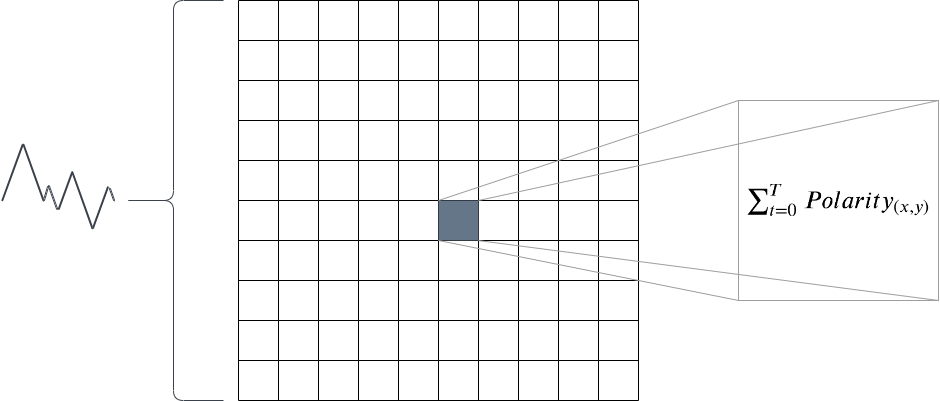
\includegraphics[width=0.8\textwidth]{analysisanddesign/images/frame_integration_illustration.png}
    \caption{An illustration of the frame integration process with custom integrating method.}
    \label{fig:frame_integration_diagram}
\end{figure}

\section{Two-phase Intensity Reconstruction Models}

In order to make use of existing highly-tested and documented computer vision techniques, intensity reconstruction models were first applied to events. For this reason a two-phase network (shown in \cref{fig:two_phase_network_pipeline}) was devised, wherein events are reconstructed into intensity videos before being passed into various classification networks. Each event stream was passed into the E2VID reconstruction network\cite{spikingToVideo}, allowing for each network that the data is fed into to analyse more complex visual patterns than are available from the frame-integrated event streams. The rationale behind this is that commonly used neural networks for video analysis are built to detect features from intensity frames rather than event streams. Therefore in order to make use of these specialisations each event stream needs to be converted into a more common input form.

\begin{figure}[htb]
    \centering
    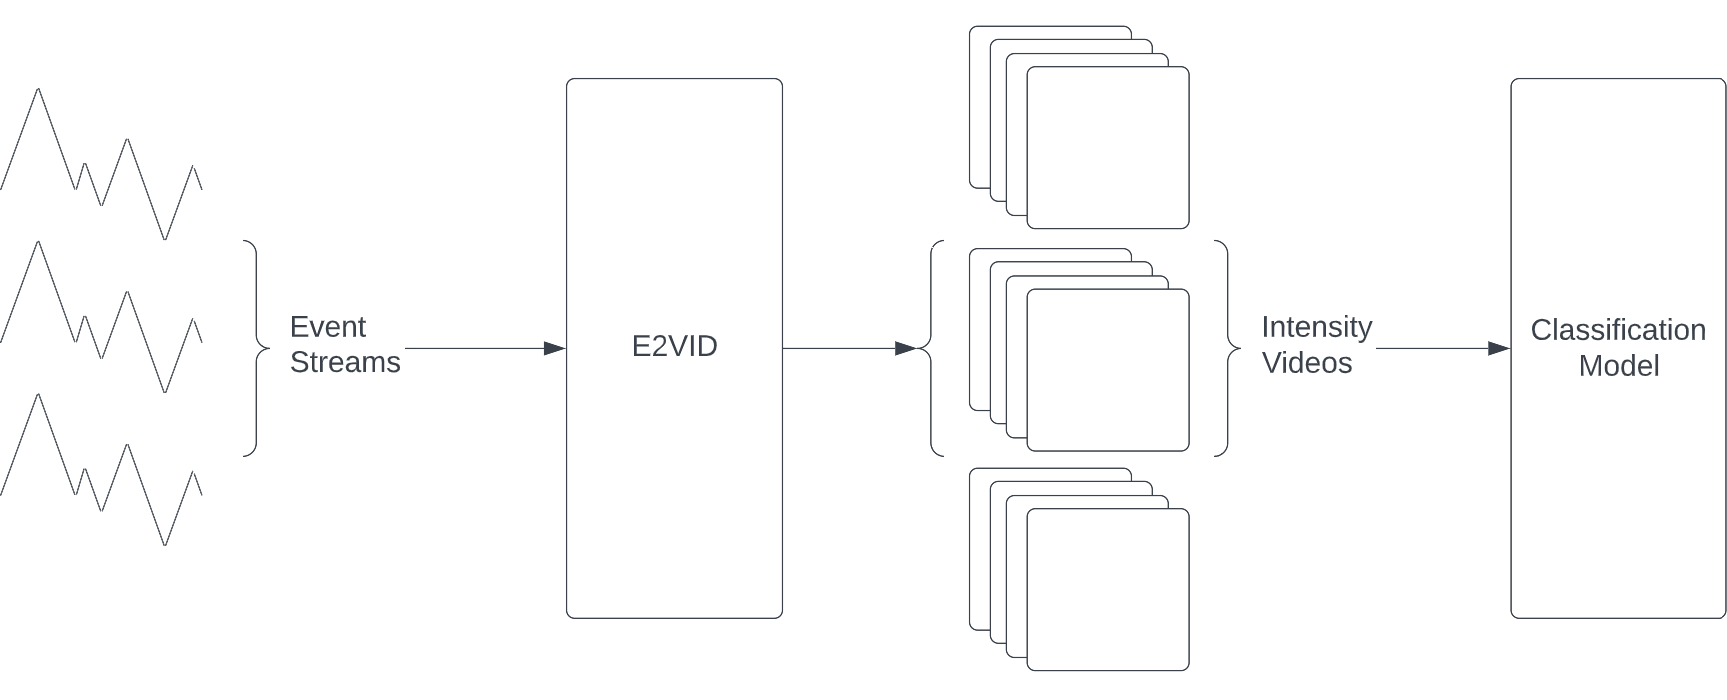
\includegraphics[width=0.85\textwidth]{analysisanddesign/images/two_phase_network_pipeline.png}
    \caption{An illustration of the two-phase classification pipeline.}
    \label{fig:two_phase_network_pipeline}
\end{figure}

\section{Classification Networks}

Given below are the various networks used to classify either integrated frames or image reconstructions. Each network has its benefits and drawbacks, but there are a few commonalities between them. 

During the training process of each of the networks a callback function was used called \lstinline{EarlyStopping}. This built-in Keras callback allows for the interrupting of network training when the validation accuracy of the network stagnates or falls, which should in theory prevent over-fitting to the training data. A patience value is set so that even if accuracy drops for only one epoch it is possible it can rise again. This, of course, means that the training data-set needs to be split into training and validation, where the validation set is more unseen data to evaluate the performance of the networks per epoch.

As well as this the most optimal weights are loaded back when the network finishes training. As well as this dropout (or recurrent dropout for LSTM and GRU cases) layers were used. These layers mean that during the training process certain neurons will be `turned off' and therefore not part of the back-propagation process. This should allow the resulting network to be robust since there is no over-reliance on any one neuron of the network.

Finally, for the learning rates for each system, it is necessary to find the optimal value. If the rate is too high, the model will quickly back-propagate to the optimal value, however once it gets close to it the weights may oscillate. This is because only a small step may be needed to make it to the ideal values, but the model constantly overshoots it. On the other hand, if the learning rate is too low, then the learning process will be very slow, and reaching an optimal value may take many epochs. As well as this, for more complex functions the network may get stuck on a local minimum value for the loss. It is clear in this case that an adaptive learning rate would be the most ideal. We would like the rate to be high to start off with, and become smaller and smaller as the training process goes on. This can be done with a Keras callback function, however for the models in this project the Adam optimiser\cite{Adam} was chosen instead. This optimiser implements a function to find the best value for the learning rate itself.

\subsection{3-Dimensional Convolutional Neural Network} \label{ssec:conv_3d_network_design}

A 3D convolutional network as described in \cref{ssec:3D_conv_network} was implemented to work on the event data. A diagram showing the function of one of the 3D convolutional layers used in the final network can be seen in \cref{fig:conv3d_diagram}. As opposed to their two dimensional counterparts, 3D convolutions involve taking video streams as input and output, allowing the network to decode patterns in both the spacial and temporal dimensions. As well as this, it the network employs batch normalisation layers accelerates training.The reason this is the case is because it provides provides some regularisation, meaning the data is rescaled so that it centres around 0 and has a standard deviation of 1. In essence this means the outputs of each intermediate layer look similar in distribution, so the same learning rate can be used for back-propagation throughout the network.

\begin{figure}[htb]
    \centering
    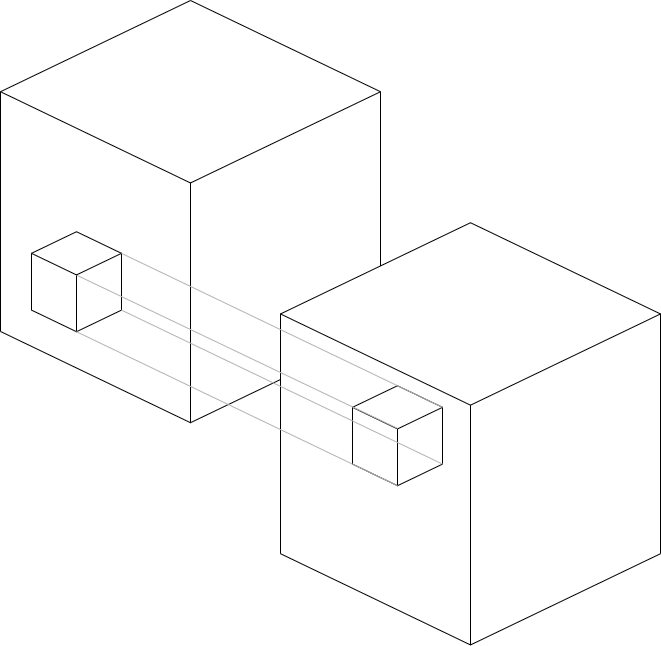
\includegraphics[width=0.4\textwidth]{analysisanddesign/images/conv3d_diagram.png}
    \caption{An illustration of a 3D convolutional layer.}
    \label{fig:conv3d_diagram}
\end{figure}

\subsection{Convolutional LSTM Network}

A convolutional LSTM network as described in \cref{ssec:conv_lstm} was implemented to work on the event data. In this network the video that is fed in is passed through the network a frame at a time. The ConvLSTM layers apply 2D convolution on the frames to extract spacial patterns, and then these features are passed into LSTMs. The LSTMs allow for the network to remember previous frames and therefore analyse temporal features of the data as well.

\subsection{Custom Convolutional LSTM Network}

This network is an extension of the LSTM network in the previous section, adding more capacity for the model to learn spatio-temporal patterns. It involves altering the intermediate convolutional neural network that analyses each frame in the video time series. A diagram showing the pipeline of the overall network can be seen in \cref{fig:custom_conv_lstm_pipeline}. This additional capacity is helpful for deciphering more complex `actions' in a video, such as in the case of gesture recognition.

\begin{figure}[htb]
    \centering
    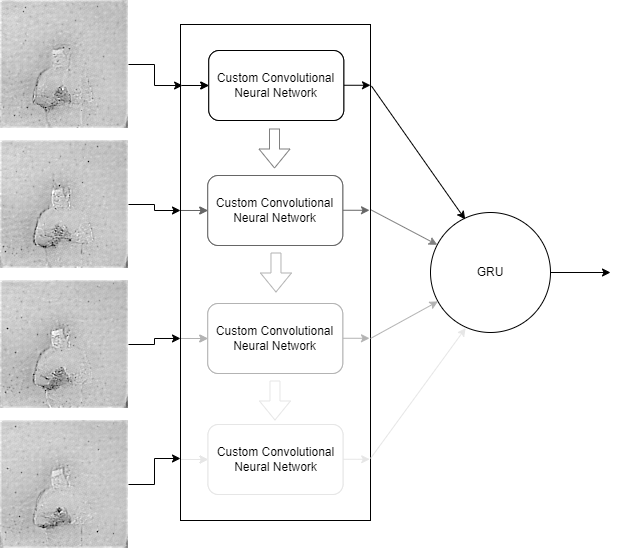
\includegraphics[width=0.65\textwidth]{analysisanddesign/images/custom_conv_lstm_pipeline.png}
    \caption{An illustration of the custom convolutional LSTM network.}
    \label{fig:custom_conv_lstm_pipeline}
\end{figure}

\subsection{Spiking Neural Network} \label{ssec:snn_design}

With this network the whole system, from data generation to classification, could be fully neuromorphic. Using techniques as described in \cref{ssec:snn_and_heterogeneity}, traditional ANNs could easily be converted to SNNs\cite{Ann2Snn} for classification. For the conversion process the \lstinline{nengo_dl} package can be used (see \cref{sssec:nengo}). In order to train the network a differentiable approximation of the spiking neurons was used. This meant that the data could be trained using back-propagation as normal. During inference, however, the actual spiking neurons could be used\cite{TrainingSnn}. Since the network is trained before the conversion from ANN to SNN, the performance of the SNN will not be comparable to the ANN due to approximation errors. These approximations can be improved by changing certain properties of the SNN and checking the performance of the inference.

Spiking neural networks work similarly to ANNs, however there are some key differences. One major difference is in the activation of the neurons. Whereas with non-spiking artificial neurons the output is a continuous function based on the instantaneous input, spiking neurons accumulate inputs and build up to an eventual spike. This means that inputs to the neuron have to be sustained (repeated) for a certain amount of time to allow for this build-up of potential. For our network, since it is a 3D vector of frames over time, the input to the network needs to be a 4D vector. An illustration of the creation of the 3D vectors that were input into the ANN and the subsequent 4D network fed into the spiking equivalent are shown in \cref{fig:sustained_video}.

\begin{figure}[htb]
    \centering
    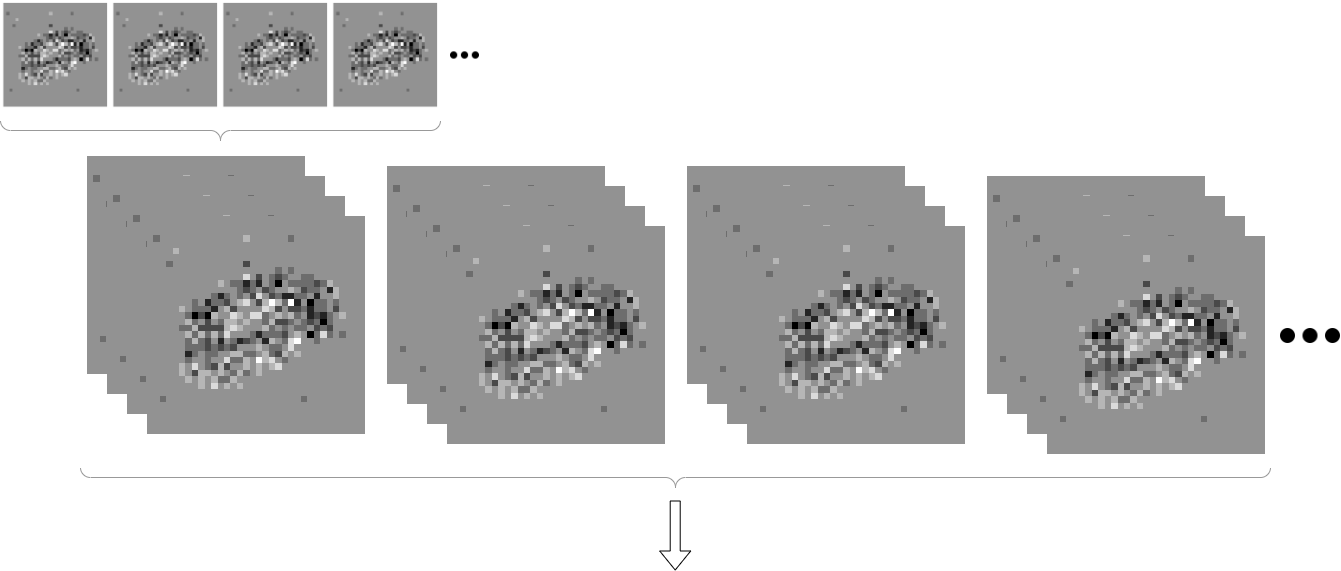
\includegraphics[width=0.75\textwidth]{analysisanddesign/images/sustained_video.png}
    \caption{An illustration of how frames of a video can be repeated for input to a spiking neural network.}
    \label{fig:sustained_video}
\end{figure}

However, unlike convolutional network layers, recurrent layers such as LSTM and GRU do not have a direct conversion available to spiking networks. There is, however, a component known as Legendre Memory Unit (LMU) that are much better suited to the conversion process. Like LSTMs, LMUs have been shown to perform as well in a variety of tasks with relatively few internal parameters\cite{LMU}. \color{red} TODO: Write more about the design of this network \color{black}.

\section{Evaluation Metrics} \label{sec:evalutaion_metrics}

The evaluation plan is as given by the typical machine learning pipeline\cite{IntroToML}.For a classification task, when we would obtain the results from the test dataset (an example of which is shown in \cref{tab:possible_results}) we can calculate a variety of evaluation metrics that give various insights on our final model.

\begin{table}[htb]
    \centering
    \begin{tabular}{|| c  | c ||}
        \hline
        Labels     & Predictions \\
        \hline \hline
        1          & 1           \\
        \hline
        1          & 2           \\
        \hline
        3          & 8           \\
        \hline
        9          & 9           \\
        \hline
        6          & 9           \\
        \hline
        $ \vdots $ & $ \vdots $  \\
    \end{tabular}
    \caption{A table showing an example of results when inputting test data from NMNIST dataset\cite{NMNIST} into the final model.}
    \label{tab:possible_results}
\end{table}

\subsection{Confusion matrix}

Confusion matrices act as a visualisation of a systems performance. It shows possible true labels as well as possible predicted labels on either side, and filled in are the number of results that fit in each segment. In \cref{tab:confusion_matrix} the confusion matrix for the NMNIST dataset is shown as an example. It should be noted that a similar confusion matrix should be created taking each class as positive, then each metric can be calculated by taking the averages (as shown in \cref{ssec:eval_metric_averaging}). For each of the cells the number of matching records are stored to calculate each of the evaluation metrics. The table includes True Positives (TP), False Positives (FP), True Negatives (TN) and False Negatives (FN).

\begin{table}[htb]
    \centering
    \begin{tabular}{|| c c | c | c | c | c ||}
        \hline
                                                                         &                                    & \multicolumn{4}{ c ||}{\textbf{Predicted Class}}                                        \\
        \cline{3-6}
                                                                         &                                    & 1                                                & 2          & 3          & $ \hdots $ \\
        \hline
        \multirow{6}{*}{\rotatebox[origin=c]{90}{\textbf{Actual Class}}} & \multicolumn{1}{| c |}{1}          & TP                                               & FN         & FN         & $ \hdots $ \\
        \cline{2-6}
                                                                         & \multicolumn{1}{| c |}{2}          & FP                                               & TN         & TN         & $ \hdots $ \\
        \cline{2-6}
                                                                         & \multicolumn{1}{| c |}{3}          & FP                                               & TN         & TN         & $ \hdots $ \\
        \cline{2-6}
                                                                         & \multicolumn{1}{| c |}{4}          & FP                                               & TN         & TN         & $ \hdots $ \\
        \cline{2-6}
                                                                         & \multicolumn{1}{| c |}{5}          & FP                                               & TN         & TN         & $ \hdots $ \\
        \cline{2-6}
                                                                         & \multicolumn{1}{| c |}{$ \vdots $} & $ \vdots $                                       & $ \vdots $ & $ \vdots $ & $ \ddots $ \\
    \end{tabular}
    \caption{a table showing one particular confusion matrix for NMNIST dataset\cite{NMNIST} for class 1 as the positive class.}
    \label{tab:confusion_matrix}
\end{table}

\subsection{Accuracy}

The accuracy of the system is the proportion of samples correctly classified.

$$ Accuracy = \frac{TP + TN}{TP + TN + FP + FN} $$

Note: classification error can also be used and is defined as $ 1 - accuracy $.

\subsection{Precision}

Precision is the proportion of positively predicted samples identified correctly.

$$ Precision = \frac{TP}{TP + FP} $$

It should be noted that a high precision may mean that there are many false positives.

\subsection{Recall}

Recall is the proportion of actual positives correctly classified.

$$ Recall = \frac{TP}{TP + FN} $$

It should be noted that a high recall may mean a lot of positive samples may be missed.

\subsection{F-measure/F-score}

This is defined as the harmonic mean of precision and recall in order to get one number as an average measure of performance.

$$ F_1 = \frac{2 \cdot precision \cdot recall}{precision + recall} $$

\subsection{Micro and Macro Averaging} \label{ssec:eval_metric_averaging}

Macro-averaging involves taking an average on the class level. Metrics are calculated for each class and then averaged at the end. Micro-averaging involves taking an average on the item level (i.e., taking the average of each of TP, FP, TN and FN to get the averages metrics).